\documentclass[runningheads]{llncs}

\usepackage[T1]{fontenc}
\usepackage{graphicx}


\begin{document}

\title{PErsoNal Genome QUery IN healthcare and clinical practice (PENGQUIN)}

\author{Elias Crum\inst{1,2}\orcidID{0009-0005-3991-754X}}
\authorrunning{E. Crum et al.}
\institute{IDLab, Department of Electronics and Information Systems, Ghent University -- imec, Belgium \and
Flemish institute for Technological Research (VITO) Mol, Belgium
}


\maketitle

\begin{abstract}
	Early Stage Ph.D. (where to put this??)

	Medical care is in the process of becoming increasingly personalized through the use of patient genetic information. 
	At present, digital data useful for clinical care is commonly diffuse, organized arbitrarily, and stored in data silos. 
	Here I propose a Ph.D. that aims to improve shareability of genomic data storage(s), while preserving data privacy, through the use of Solid pods. 
	I also propose plans to investigate representing personal genome sequence data in Resourse Description Format as Linked Data, where linkages are representative of semantic, medically relevant data.
	To make such a storage framework clinically useful, I aim to evaluate the how queries over this Linked genomic Data could be executed using a query engine approach.
	Preliminarily, I have succeeded in storing genomic data in representative patient data pods using Solid specifications. 
	I aim to show in future work that this novel appraoch to storing clinical patient genomic data improves clinical data sharibility, discoverability, and data flow efficiency through the use of Linked Data formats and querying infrastructre. 

\keywords{Solid \and Linked Data \and Querying \and Genomic Data Sharing.}

\end{abstract}


\section{Introduction / Motivation}
\textit{Give a general introduction to the domain/area/topic and indication of its importance/impact in Semantic Web research or other domains.} 

As our understanding of genomics deepens, the role of Personal Genome Sequencing (PGS) in healthcare becomes increasingly vital. 
At the time of writing, there are multiple domains of clinical practice where patient PGS data is used to inform medical decision making \cite{souche_recommendations_2022, gil_analysis_2015}. 
For over a decade, PGS data has been poised to be scaled to generalized clinical practice, but at present this is largely not the case \cite{alzubi_personal_2014}. 
While there are many documented challenges to wider clinical implementation of personalized medicine \cite{stefanicka-wojtas_barriers_2023}, one major challenge is presented by the digital representation, storage, and access to the PGS data that underlies all personalized medicine workflows.
With this project, I aim to address the challenges presented by PGS data usage in clinical practice through the use of emerging decentralized storage and querying technologies.  


\subsection{Medical Motivations for PGS data in Cinical Practice}
At present, there are major medical fields that preliminarily show readiness for and benefit from greater use of PGS data, these being drug development and prescription, cancer diagnosis and treatment, and rare genetic disease identification and treatment.
Genomic variation is thought to account for up to 95\% of outcome variations in drug prescription and treatment efficacy \cite{belle_genetic_2008}, while also becoming informative for new drug development recently \cite{ko_new_2022}. 
In clinical practice, studies have documented genotype correlation with unintended drug responses for commonly prescribed drugs such as warfarin \cite{linder_genetic_2001} and many others \cite{research_table_2024}. 
PGS usage, by helping predict, better understand, and inform optimal drug treatment plans, shows great potential for improving on the one-size-fits-all, trial and error approach to drug prescription popularly practiced today \cite{hens_return_2011}. 
Similarily, for cancer patients, the use of PGS data has been shown to augment existing strategies of diagnosis and treatment \cite{mcleod_cancer_2013}. 
One of the most developed, wide-spread implementions of PGS data usage in clinical practice is in rare genetic disease identification and treatment \cite{krier_genomic_2016}. 
Despite these advanced use cases, barriers to adoption remain, especially due to the cost and technological infrastructure demands posed by large scale PGS data generation, storage, and analysis.


\subsection{PGS data storage and sharing}. 
Talk about - 
why data storage is important, 
why data sharing is important,

Within clinical practice, the key concerns related to PGS data storage and sharing are presented by three major constituents of the clinical ecosystem, those of the \textbf{patient, clinician, and healthcare administration}. 


From \textbf{all three perspectives}, privacy is of the utmost importance. 
While there is open debate about the degree to which patients should be able to control their own personal medical data \cite{blumenthal_giving_2015,damen_patients_2022}, legally, within the European Union, a core tenant of current personal data usage is transparency \cite{spagnuelo_qualifying_2020}. 
Protections for citizens relating to sensitive personal data are codified in the European Union\textquotesingle s General Data Protection Regulation (GDPR) law, since 2018 \cite{noauthor_regulation_2016}. 
PGS data, along with other health-related data, is categorized as “sensitive” data in the GDPR, carrying with it the strictest privacy safeguards. 

From the perspective of \textbf{the patient}, 
awareness and control over their personal data usage is a consideration that the current system does not much address. 
As established by the GDPR, technical infrastructure designed for the storage and accessing of PGS data requires special attention to methodologies that address patient control and/or transparency over usage of their data. 
Because of the architecture of centralized databases, granular permissions for specific subsets of sensitive data are challenging to implement yet could allow for a patient to view their own PGS data, thus improving their connection to their own personal data. 
Additionally, policy implementations such as patient ability to view and/or approve or deny consent to PGS data usage for specific instances, rather than a blanket consent at time of collection, will improve the patient\textquotesingle s involvement in how their data is used. 

From the perspective of \textbf{the clinician}, being able to access patient data, share patient data with providers outside one medical institution\textquotesingle s system, and not need to worry about data interoperability with biomedical tools, applications, or user interfaces is crucial. 
Data interoperability challenges emerge from the complex process of generating and storing PGS data as well as the large size of these datasets. 
The average human genome is slightly over 3 billion base pairs in length (3 Gbp). 
During a whole genome sequencing workflow, various sequence formats, that offer different sets of information, such as FASTQ \cite{cock_sanger_2010}, SAM/BAM/CRAM \cite{li_sequence_2009, bonfield_cram_2022}, VCF \cite{danecek_variant_2011}, and others are produced. 
With respect to clinical practice, the VCF file offers genomic information most useful to most current clinical applications. <-- bad sentence
VCF files are typically between 100-1000s MB (0.1-1 GB) in size within computer memory when compressed and represent ~10^6 nucleotide positions of an individual\textquotesingle s PGS. 
While these data formats are widely considered the state-of-the-art for most genomic data applicaitons, often the organization-specific directory structure and file naming protocol makes PGS data non-interoperable between databases.

From the perspective of \textbf{healthcare administration}, the cost of generating, storing, and maintaining patient PGS data, with the necessary privacy protections and monitoring, is nontrivial. 
The result is little data sharing between institutions, or even within divisions of the same institution.
Therefore, institutions are responsible for re-generating PGS data for patients from out-of-network regardless of whether they may have an already generated genome sequence at another institution. 
Such data duplication represents unnecessary inefficiency that costs both the patient and institution, especially due to the heavy computational demands in generating PGS data and the high storage demands for the large PGS data files produced. 
During the life of that data, the hospital system that maintains the storage is also responsible for preserving the privacy of that information. 





\textbf{Resource Description Format (RDF) and Linked Data}
RDF is a way of representing data that allows for data linking...
It is useful for representing semantic relationships between data ...
Many public biological databases have been converted to RDF because of its advantages for data querying + linking...
RDF holds promise within healthcare for concentrating medically-relevant data (through linkages)
no clinical implementations yet

\textbf{Link Traversal Query Processing}
Querying RDF and linked data is very different than relational databases...
Approaches for such data querying have been proposed, but not for genomic or medical data...
Popular algorithms that may provide usable results are ...

\textbf{Project Motivation}
Despite there being no real options for clinical PGS data sharing at present, there is also a conspicuous gap in the current scientific discourse around the development and implementation of such a infrastructure for personal genome data sharing for clinical use. 
This gap underscores the necessity of the proposed doctoral research project.
Our aim is to develop Personal Genome Pods using the Solid protocol[c], a set of technical specifications that enables decentralized data storage and infrastructure for data privacy preservation alongside increased sharing capabilities.  
I envisage that this project will significantly contribute to the field of personalized medicine and clinical genomic research by empowering individuals to utilize their personal genomes in healthcare and clinical practice in a manner that reinforces their autonomy and privacy. 
My project described here will aim to establish the feasibility of using decentralized storage technologies for PGS data storage and sharing with the hope that it results in direct translation into a product and/or acts as the schematic upon which future products are based. 


We aim to link PGS data to other patient data stored within the same pod, publicly available external databases containing pertinent data, and/or other patient data within separate Solid pods, discoverable to those with authorization.


\section{State of the Art}
\textit{Describe existing work in the area, work focusing on the same/similar problems or that might be useful to tackling your research question.}

\subsection{Current State of the Art -- Clinical data storage}
Presently, most clinically relevant health data is stored using an \underline{institution-centric approach}, including PGS data. 
This strategy is characterized by the hospital or hospital system isolating all of its stored data into one or more centralized databases that are governed and maintained solely by the owner institution. 
Here, centralized storage is defined as the structural organization of a data store, establishing that a single node, the system that hosts the physical data storage, has control over managing database content, access, and permissions. 
With this system, healthcare institutions prioritize patient data privacy over all other digital data storage considerations. 
By prioritizing patient data privacy, access is commonly only allowed for authorized users within the institution\textquotesingle s internal network. 
Crucially, this institution-centric data storage architecture, by design, allows for little to no accessibility for users or data usage requests that originate outside of the institution\textquotesingle s network, largely due to the organizational design of such centralized data storage systems. 
With the enlarged threat of hacking, phishing, and login credential compromisation that seems to only be increasing \cite{noauthor_ransomware_nodate}, hospitals and institutions that maintain patient PGS data are forced to enact tighter regulation over data access within their institution, severely limit outside institution access, and increase the in-house cyber security staff or pay for external companies to handle such security audits.  
Due to this isolation of patient PGS data to a single institution, data duplication leading to increased storage and data generation costs, severely limited patient data usage transparency, and severely limited potential for data sharing are observed. 
Collectively, these state-of-the-art approaches to PGS data storage inhibit the scalability of PGS data usage in the above discussed clinical applications due to raising PGS usage costs.


\textbf{Current State of the Art -- Clinical}
As discussed above, there are some current use cases for PGS data clinical workflows, and thus, state-of-the-art systems established for  patient PGS data storage and access. 
Importantly, like other health data, clinical PGS data is stored using an \underline{institution-centric approach}. 
This strategy is characterized by the hospital or hospital system isolating all its stored data into one or more centralized databases that are governed and maintained solely by the owner institution. 
Here, centralized storage is defined as the structural organization of a data store, establishing that a single node, the system that hosts the physical data storage, has control over managing database content, access, and permissions. 
With this system, healthcare institutions prioritize patient data privacy over all other digital data storage conditions. 
This method of data storage prioritizes patient data security and access only for authorized users within the institution\textquotesingle s internal network. 
Crucially, this institution-centric data storage architecture, by design, allows for little to no accessibility for users or data usage requests that originate outside of the institution\textquotesingle s network, largely due to the organizational design of such centralized data storage systems. 
With the enlarged threat of hacking, phishing, and login credential compromisation that seems to only be increasing[c], hospitals and institutions that maintain patient PGS data are forced to enact tighter regulation over data access within their institution, severely limit outside institution access, and increase the in-house cyber security staff or pay for external companies to handle such security audits.  
Due to this isolation of patient PGS data to a single institution, data duplication leading to increased storage and data generation costs, severely limited patient data usage transparency, and severely limited potential for data sharing are observed. 
Collectively, these state-of-the-art approaches to PGS data storage inhibit the scalability of PGS data usage in the above discussed clinical applications due to raising PGS usage costs.

\textbf{Current State of the Art -- Academic Reserach and Consumer Market}
Apart from the current practices within healthcare institutions, other approaches for consumer access to their PGS data by private companies, PGS data sharing between research institutions, and general health data interoperability initiatives by multi-institution consortiums have been innovating the ways PGS data is stored and shared. 

Private companies, such as 23andMe, Ancestry.com, Sequencing.com, and others, offer consumption-centered genomic products such as ancestry profiles, health risk screenings, and rare-disease management guidelines among other emerging services. 
Such services have highlighted a public interest in being able to see and access their PGS data as well as learn useful things about themselves from it.
This emerging market reflects that consumers are keen to be able to access their PGS data, or at least use such data to know more about themselves. 
At the same time, innovation in this niche is not situated to handle the challenges presented by PGS data in clinical practice. 
Between similar centralized data storage approaches to hospital systems and large data leaks for companies like 23andMe in recent years, the prospect of existing companies offering solutions attractive enough to convince consumers or hospital systems to adopt a new system is unlikely. 

In the realm of academic reserach, the development of infrastructure that allows for sharing of genome data between institutions has gained traction recently. 
Due to reasons related to patient data privacy preservation, data is predominantly anonymized for sharing to be admissible. 
Initiatives such as OHDSI OMOP, HL7 FHIR, GA4GH Beacons, and others are building the infrastructure and establishing the interoperability standards necessary for between institution data sharing in this manner. 
The major drawbacks of these proposed solutions are, (a) the requirement that data must be anonymized for true sharing or, (b) control of data analysis is relinquished to the data\textquotesingle s home institution, thereby establishing federated networks of hospital data for data discoverability, but restricting actual access to such data for privacy reasons.

Despite great progress in research and consumer domains, advancements in state-of-the-art infrastructure and standards are not directly translatable to clinical practice due to various cinically unique demands detailed in the introduction. 


\textbf{Alternative Solutions}
A conceptual approach that offers a solution for the current challenges in data privacy, accessibility, and interoperability is moving away from an institution-centric model for PGS data storage and toward a citizen-centric one. More broadly, initiatives that exist in the health data domain are advocating for a similar change in technological philosophy. While this movement is still in its early stages, calls for leveraging decentralized storage technologies such as Solid, ..., ..., or Block Chain, have been proposed[c]. While there is still much work to be done before these fledgling technologies could be applied in practice, such approaches to PGS data storage offer great promise because of their ability to offer citizen-centric storage while also hosting the building blocks for features such as consent-driven data sharing, granularized data policy enforcement, stored data representation as Linked Data, and authorized data access over the web to just name some possibilities. 


\section{Problem Statement and Contributions}
\textit{Formulate the problem you intend to solve, and how you intend to contribute to Semantic Web research. This section should include a clear formulation of one (or very few) research hypothesis (what statement you want to validate through your methodology, approach and evaluation), and/or the research questions that need to be answered.}

My research project is situated to provide a proof-of-concept PGS data storage and sharing framework that can be adapted to use for clinical practice. In this pursuit, my core research questions are: 
(A) Can a citizen-centric PGS data storage framework, developed using a decentralized storage technology, offer data sharing infrastructure while maintaining privacy safeguards for sensitive data? 
(B) Can the PGS data be stored as RDF, be linked to other medically-relevant data, and be queried over in a way acceptable for use by medical professionals? (<-- not great, need to improve wording)
To address these central questions, I will investigate the use of data pods, implemented using Solid protocol, to store PGS data in a decentralized and privacy-oriented ecosystem while addressing technical challenges associated with data policies, representation of PGS data as Linked Data, discoverability through querying, and infrastructure that connects data pods to existing clinical workflows and tools. 
My hypothesis is that such a framework can be developed and would offer unique advantages over the existing state-of-the-art institution-centric PGS data storage solutions. 
The following six objectives will be undertaken to test my hypostheses through experimental production and testing of different modules of the proposed framework.

(1) \textbf{Identify the workflows, tools, and data networks that utilize PGS data for framework connection.}
_What: Assess the current state-of-the-art in the field of clinical PGS data formatting, usage, and sharing. 
Describe existing methods used for PGS storage, PGS data sharing, and PGS data integration into clinical workflows.
_Result: Establish tangible goals for how my framework can be implemented into existing workflows and initiatives. These goals will inform the architecture of the framework and how future implementations are deployed. 
_Challenging: There are many initiatives, standards, and potenital clinical workflow applications that have different data formatting standards, technical requirements, and implementation specifications. 
_Why me: My education in bioinformatics, past research in genomics, and work experience in clinical settings has provided me with the tools and skills necessary to parse the many options and select those that will offer high impact and fit most seamlessly with the proposed framework.


(2) \textbf{Solid Pod PGS Data Storage.}
_What: Develop methods and a workflow for the creation and hosting of individual patient Solid pods as well as the transfer of PGS data, primarily in vcf file format, into those Solid data pods. 
_Result: I will produce a proof-of-concept demo that exhibits that the Solid decentralized data storage ecosystem can be implemented and host PGS data in a citizen-centric architecture.
_Challenging: Such a framework for genome data has not been undertaken before in the literature and most past implementations of Solid data pod use cases have not been designed to handle the large data files that are presented by PGS data. 
_why me: ???


(3) \textbf{Data formatting and interoperability.} 
_What: I will experiment with the conversion of PGS data from vcf files to RDF serialized in ttl file format. 
We intend to investigate the viability of representing VCF file data as Linked Data which necesssitates the mapping from this biological file format, vcf, to RDF. 
_Result: I aim to make such a mapping process bi-directional because most existing clinical workflows necessitate input files in VCF, thereby making a returnable VCF file on request necessary. 
Thus, an index file will be maintained for VCF to RDF conversion bidirectionally.
_Challenging: The conversion between VCF and RDF will require the use of an ontology and computation. 
Decisions regarding how the computation will be done, when the computation will be done, and what exact computation will be performed are all open questions.
I will assess the computational demands of the conversion process as well as the storage costs of the RDF files produced to optimize the storage and conversion strategies.


(4) \textbf{Data policy and accessing.} 
_What: A fundamental goal of any PGS data storage system is mainting the privacy of the stored PGS data. 
I will investigate the ways in which data access requests, data usage consent, and granularization of consent to particular pieces of data can be applied to PGS data stored in Solid pods.
_Result: I will develop methods within the larger framework for data to be accessed by authorized users, adding and changing restrictions for access, requests for access by clinical professionals or researchers, and access controls that function at a level lower that the pod owner's whole pod.
_Challenging: There are trade-offs between privacy and accessibility, and ultimately, the addition of privacy considerations to data will have the most impact on quering the data within a pod...
_why me: I have direct experience with health care systems in the USA and am familiar with challenges associated with privacy protection strategies used for sensitive health data. 
I plan to apply this knowledge in the design of a system for privacy protections that is intuitive to users and provides more granular privacy options than the current systems available. 

(5) \textbf{Data querying}
_What: Investigate query processing techniques for a single and across multiple Solid pods containing PGS data. 
Assess the efficacy of existing querying algorithms applied to PGS data in both RDF and vcf formats and compare results to common vcf parsing tools publicly available.
_Result: Develop performant query strategies for Solid pods containing PGS data.
_Challenging: PGS data is large, in particular, vcf files are 100-1000s MBs in size, thus, performant querying can present a challenge. Additional complexity will be introduced to querying PGS data formatted as Linked Data.
_why me: My background in genomics and bioiformatics can help me both assess and innovate existing approaches to RDF and Linked Data querying approaches.

\ec{This is a question I do not know how to answer right now --> What is lacking in existing query algos that necessitate you to build new ones?}


(6) \textbf{Framework unification and deployment}
Together, these objectives will be combined into an operational framework that uses the proposed methods for storing, protecting, sharing, and querying PGS data for clinical use. The framework, once produced, will be comapred to existing strategies for storing and sharing PGS data to assess the efficacy of transitioning toward product production and marketing.


The proposed scientific approach will contribute novel data and conclusions to numerous fields of semantic web research. These findings will include an approach to how decentralized storage specifications can be applied to store sensitive medical data, how genomic and medical data can be represented and queried as Linked Data, how existing Linked Data querying algorithms perform over genomic and health data, ..., 



\section{Research Methodology and Approach}
\textit{Describe the research methodology you will apply in your research, including the different steps from the formulation of your research questions to answering them. Also describe the approach you are taking (or you intend to take for Early Stage Ph.D. submissions) to instantiate the research methodology, hence contributing to solve the problem described in Section 3 and confirm or reject your hypothesis. Discuss how this approach is innovative and novel, and how it is (might be) implemented.}

My project will be split into five different component work packages and a final sixth work package where the components will be deployed as a cohesive framework. The workpackages will be worked on relatively linearly and specific milestones are outlined below.


\begin{figure}
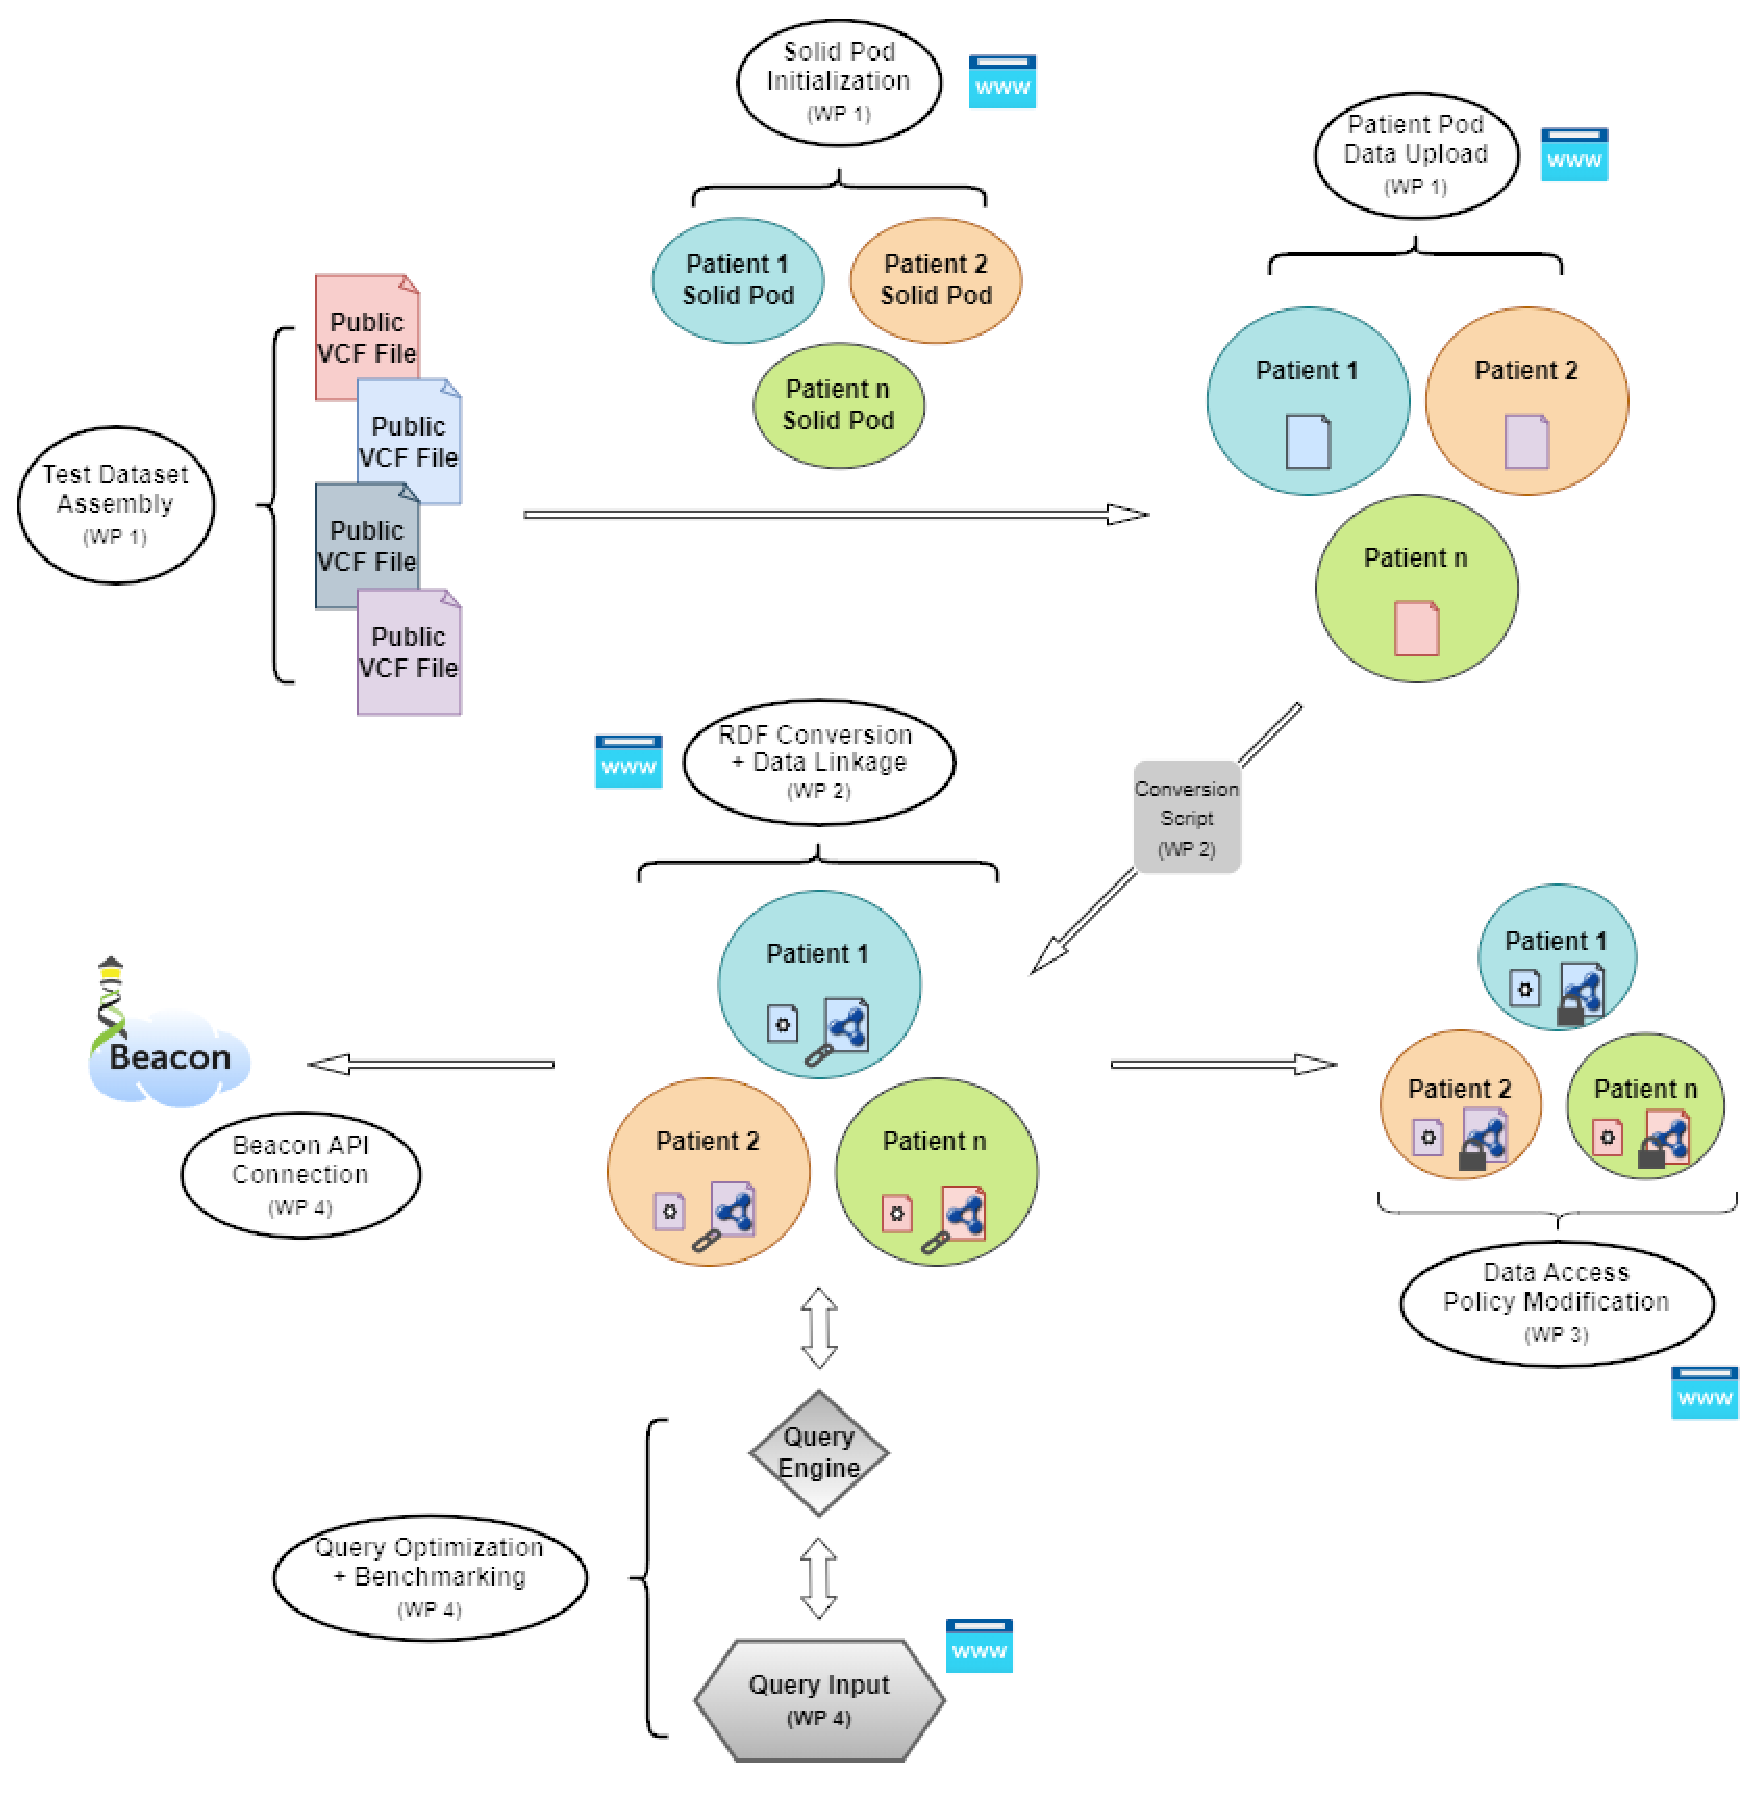
\includegraphics[width=\textwidth]{fig1.eps}
\caption{Figure 1 PENGQUIN project workflow.
White circles represent locations within the workflow where objectives will be achieved. 
For each of the steps in the workflow, the work packages affecting this step are also shown in parentheses (if applicable). 
This workflow is slightly oversimplified for ease of understanding the project.
} \label{fig1}
\end{figure}

\subsection{Work Package 1: Establishing the practical connection goals that encourage clinical use}

- Scoping review (storage / sharing approaches that exist)
- File types (WGS and clinically relevant file types)
- Practical use cases (what types of input data do they require / how are results reported)
- What technological foundations will be necessary?

To establish the practical use cases upon which to design my project, I will begin my Ph.D. project by writing a scoping review paper that details the ways in which PGS data are currently used in clinical practice as well as the tools and systems currently in place to facilitate the storage and sharing of these PGS data. 
Along with assessing the current use cases for PGS data in clinical practice, I will also investigate the input file and data formats necessary for these pipelines and tools. I will specifically focus on whole genome sequencing file types, as these are the most promising for future applications. 
Finally, I will determine the viablility of decentralized storage systems for use in PGS data storage and sharing as well as ...

I will conduct a literature review of: the Solid decentralized data storage framework, secure/confidential data storage in decentralized environments, existing human genome single nucleotide polymorphism summary file (.vcf files) parsing approaches. A review of these aims has not been performed before and is aimed at representing the state-of-the-art of various areas within the field of PGS data sharing.

Importantly, I aim to for this framework to facilitate the greater access of PGS data to both existing and future applications and clinical tools. 
To accomplish this generalizability, I will investigate popular ongoing health data initiatives aimed at standardizing genomic data formats and directory structures, establishing queryable, federated networks of health and genomic data, and (another thing here?)

In an effort to improve data flows for research purposes, I intend to connect the proposed framework to the international Beacon initiative[c,c] to increase the availability and ease of access of genomic data for researchers globally. 
In this aim we will make patient PGS data beacon endpoints that can be discoverable abd queried via the Beacon API.
This option to contribute personal genomic data to the greater Beacon data network, thereby making it discoverable to researchers, will be controllable on an individual basis as an opt-in option. 
The connection of a decentralized storage framework to the Beacon network is novel in nature as all other existing endpoints are relational databases maintained by hospitals or research institutions.


\textbf{Milestones:} 
\begin{enumerate}
	\item Literature review of existing genome storage implementations
	\item Scoping review paper composition
	\item Submission for paper publication in a peer-reviewed journal
	\item Determination of preliminary use case goals
	\item Format standards for initial implementations
\end{enumerate}

\textbf{Risks and Mitigation:}  
\begin{itemize}
	\item \textbf{Paper is not accepted:} if the scoping review paper is not accepted for publication for a journal article, I will investigate alternative methods of publication such as conferences, paper recomposition for a different purpose, or some other alternative that allows for communication of results.
	\item \textbf{Approach and/or underlying goals change:} under close advisement of my Ph.D. promoters, we will formulate a new apprach that addresses barriers to progress or success that arise from unforseen circumstances or changes in current field of scientific investigation.
\end{itemize}

\subsection{Work Package 2: Storing and publishing personal genomic data in a decentralized environment} 

- Set up solid pods using the CSS
- Create an interface for data management and uploading
- Make a test dataset of PGS data for future experimentation

In this work package, I will set up the technical foundations for experimentation that will continue in later work packages. 
A test dataset will be constructed using publicly available Illumina platinum genome files[c]. 
These files will be used as representative "patient" PGS data for early stages of the project. 
There are 13 individuals\textquotesingle  PGS data represented in this dataset. 
All data described here is publicly available and can be found here[c]. 
In later stages of the project, additional publicly available and/or AI generated PGS data may be utilized to test the performance of the framework when scaled to hundreds or thousands of pods, but this will be assessed later in the Ph.D. project. 

Within this work package, I will also create server-hosted Solid pods that are representative of individual patient Solid pods using the Community Solid Server (CSS) specifications. 
Each pod will be a storage container for a single individual\textquotesingle s PGS data. 
The pods will be first hosted on a local machine as a server to establish a proof of concept.
After initial hosting locally, a dedicated server will be set up for hosting a large number of pods for the duration of the project. 
We thus create a representative patient\textquotesingle s pod and upload a single PGS file, a vcf file to start, into that pod to test basic functionality of a Solid pod for hosting patient data. Once this is demonstrated for a single pod, the process will be testing for many pods, all using unique publicly available PGS data. Data will be uploaded and viewed using scripts that utilize HTTP requests.  
The use of the CSS for Solid pod hosting is state-of-the-art, but there have been no published experiments documenting the use of Solid pods for storing PGS data. 


\textbf{Milestones:}  
\begin{enumerate}
	\item Assemble a test dataset consisting of publicly available PGS data
	\item Create and host Solid pod(s) using the CSS specifications
	\item Develop a simple user interface for PGS data uploading and viewing for Solid Pods
\end{enumerate}

\textbf{Risks and Mitigation:} 
\begin{itemize}
	\item \textbf{Software Dependencies:} Various software will be used for this project. Generally, software is known to exhibit issues concerning quality, versioning, and documentation. If such problems are encountered troubleshooting will include utilizing other, comparable software to accomplish the task or contacting the producer of said software for troubleshooting.
	\item \textbf{The Solid protocol or CSS specifications are insufficient for envisioned development:} There are various colleagues at UGent who are involved in the active Solid community as well as maintain services such as the CSS. These colleagues will be utilized if such challenges are encountered. Additionally, CSS is an open source project that allows for personal modifications for instances where alternations must be made to satisfy particular demands. 
\end{itemize}


\subsection{Work Package 3:  Storing PGS data as RDF}

- choose an ontology for the conversion of VCF formatted PGS data to RDF
- benchmark the computational costs of this conversion
- develop strategies to efficiently convert between these two formats
- begin experimentation with linking *other* (what kinds??) patient data to PGS data

methods of ingesting non-rdf data into rdf data for storage in Solid pods

PGS data represented in vcf file format, is the most commonly used PGS data format for clinical pipeline and tool inputs. 
Therefore, I intend on making a patient\textquotesingle s PGS data discoverable in this state-of-the-art vcf format to enable connection to these existing workflows. 
As of yet, there have been few documented investigations into representing PGS data, particularly vcf files, in RDF. 
This relatively novel formatting would allow for a number of possibly advantageous data properties. 
First, any particular part of a patient\textquotesingle s genome that is represented in the vcf file could be linked to other data such as a perviuos test result, a documented protein folding error, a published pharmacogenomics directive, or a known rare genetic disease marker, among many other examples.
The power of linking the vcf data to other clinically relevant data is then realized when these semantic links can be discovered during querying. 
Second, queries across multiple patient pods can be performed and results can be obtained despite these data being stored in separate, secure locations (<-- not the right word).
While Linked Data and Linked Data Query Traversal algorithms are state-of-the-art, these appraoches have not as of yet been applied to genomics data or healthcare.

To achieve the representation of PGS data, in vcf files, as RDF, we will investigate a format conversion process using the SPHN RDF ontology to serialize PGS data in turtle (ttl) format. 
During this translation process, we will experiment with different approaches for maintaining the ability map between the vcf and RDF to maintain maximum compatability while experimenting with representing PGS data as RDF. 
This experimentation may include storing a bidirectional mapping index, both RDF and vcf files, or on-the-fly conversion of vcf to RDF during query execution. 
Additional optimization may also look into different fragmentation strategies for seralizing PGS data in separate files or other organizations that could help improve performance of RDF storage and querying.
Furthermore, I will compare the performance of the proposed mapping strategies in terms of ingestion speed, storage size, and query performance. 
Because representation of VCF files in RDF have not be heavily studied, these will be the first experiments of their kind.




Additionally, there is promise in representing genomic data as a graph as is reflected in recent advances in reference pangenome representations[c]. 

\textbf{Milestones:} 
\begin{enumerate}
	\item Create and document data format conversion method (first from VCF to RDF)
	\item Benchmark the computational and storage requirements of format conversion
	\item Experiment with the various methods of backwards conversion
	\item Benchmark the computational, time, and storage costs of various methods
	\item Integrate a method for users or applications to request a vcf file into the framework
\end{enumerate}

\textbf{Risks and Mitigation:} 
\begin{itemize}
	\item \textbf{Evolving PGS Technological Advances:} 
	Long read sequencing has been decreasing in price in recent years and offers many advantages over the currently most common form of short-read shotgun genome sequencing. 
	With a widespread transition to long read sequencing, the way downstream genomic files, such as VCF files, are created and formatted may change. 
	It is unlikely that such a drastic change will take place during this Ph.D. project, but if such a breakthrough occurs, the Ph.D. candidate and advisors will assess altering the input genomic files to align with the project\textquotesingle s goal of creating a framework useful for advancing personalized healthcare.
	\item \textbf{Existing ontology descriptions are insufficient for conversion to RDF:} If the SPHN RDF ontology is unfit for converting VCF to RDF or it becomes no longer publicly available, I will look for other published ontologies that could be used for conversion.
	If a suitable ontology cannot be found, I will work with colleagues to define and publish my own genomic ontology for use in conversting VCF to RDF.
	\item \textbf{Software Dependencies:} Various software will be used for this project. Generally, software is known to exhibit issues concerning quality, versioning, and documentation. 
	If such problems are encountered troubleshooting will include utilizing other, comparable software to accomplish the task or contacting the producer of said software for troubleshooting.
\end{itemize}


\subsection{Work Package 4: The policies for preserving PGS data privacy}

PGS data intended to be used in clinical practice is highly private and protected by legal guidelines like the GDPR. 
I will experiment with the design and implemention of methods that allow for dynamic control over data discoverability, read/write access, and requesting consent for data access stored in Solid pods.
There are three methods that are crucial to my citizen-centric PGS data storage framework.
First, a method that allows for registering the pod to an individual patient, thereby giving them read-only access to their raw PGS data through registration of an account.
Second, a method that allows for physicians or researchers to see what data is present within a patient\textquotesingle s pod, without being able to access the data itself. 
Then a method for them to request patient consent to access the actual PGS data. 
This method involves the submission of the request from the provider, the notification of the patient, and the consent or denial by the patient.
Third, a method where the patient can rescind permission for access to their data as well as an opt-in option to share their data with researchers. 
All of these methods should be accessible to the patient and provider within a simple, intuitive user interface.

Additionally, there should be additional nuances added that offer various levels of access to data read and write privelages which reflect the needs and roles of various contributers to a PGS clinical workflow. 
The data producer (sequencing facility or health data officer at a hospital) should be given the privelages to edit and add all data. 
The physician should be given privelages to add data, edit any data they have added, and view all data for their patient.
The patient should have view access for all data within their pods but no edit access.
The patient should also be given the privelage to edit permissions (other than some cases) as well as be able to transparently view all users who have access to each stored piece of data.
Any auxillary provider should have the ability to see what data is present in a patient's pod, the ability to request data access, but not default data access.
A registered reseracher should have limited access to stored data, when patients opt in to allow it, in a format that does not reflect the personal information of the patient (maybe? --> will need to play with card#me publicity)
It should be noted that these privacy restrictions are only to represent the nuanced ways in which permissions can be controlled and reflected within the framework schema.
For any product, governance over who can access and edit which data will require expert review and legal consultation. 

Assigning the above permissions within Solid is an open area of research and there are currently some state-of-the-art protocols for similar implementations. The described access schema has not been attempted in the presented level of detail for genomic data.


\textbf{Tasks:} 
\begin{enumerate}
	\item Develop documentation for patient Pod registration
	\item Define roles of Patient, Medical Professional (direct), Medical Professional (aux), Data Officer, Researcher, etc.
	\item Assign permissions to the various roles
	\item Create method for requesting consent for data access, notification of patient, and form for patient to give or deny access
	\item Create method for patient to opt-in to data sharing with researchers (with anonymization?)
	\item Implement simple interface for the patient to rescind data access
\end{enumerate}

\textbf{Risks and Mitigation:} 
\begin{itemize}
	\item \textbf{Unsure...:}
\end{itemize}


\subsection{Work Package 5: Querying over PGS data in one and many pods}

- how is data discovered in a pod?
- benchmarking with different linked data fragment traversal algorithms
- experimentation with client vs server computation for query performance
- compare performance to existing VCF parsing algorithms

This work package will build upon the storage, RDF representation, and access controls of PGS data in patient Solid data pods from the previous work packages. 
I aim to execute queries across PGS data contained within a single data pod or spread over multiple data pods through the use of the query protocol SPARQL[c]. 
PGS data serialized as RDF are essentially represented as a collection of nodes interlinked directly or indirectly as a knowledge graph which allows unique query approaches for fetching specific information. 
For this querying, a source of computation is required because Solid pods do not have any computation instrinsically attached to the stored data.
I intend to utilize a query engine approach to query execution, such as is presented by Comunica[c], for executing queries over patient Solid pods. 
For usability accross various future implemetations of the framework, I will experiment with the use of sever-side computation offered by a high performance computing center at VITO NV as well as client side browser computation for these queries.

For PGS data querying, we will benchmark and potentially build upon the link traversal query processing (LTQP) paradigm, which has been shown to be an effective method for querying within a decentralized environment such as Solid[c]. 
LTQP is known to currently perform sub-optimally for larger dataset sizes and complex queries. 
We expect that some use cases may present challenges within the PGS data space in which this will be the case. 
As such, we will look to innovate and improve performance by combining existing algorithms with strategies that leverage the unique structure of PGS data.
One strategy that I may be investigate is the use of pre-computed indexes, that are also used for RDF to VCF conversion, as a guide for faster query processing.
Various approaches will be developed and assessed on a population of PGS data pods through benchmarking to compare query performance. 

\textbf{Tasks:} 
\begin{enumerate}
	\item Establish that PGS data within a Solid pod can be queried using SPARQL via a query engine
	\item Benchmark how computational source impacts PGS data query perfomance
	\item Benchmark queries over single and multiple pod PGS data using existing LTQP algorithms
	\item Develop novel algorithmic approach using pre-computed indexes and compare to LTQP algorithms
	\item Integrate query functionality into a user interface (with example queries for non-experts)
\end{enumerate}

\textbf{Risks and Mitigation:} 
\begin{itemize}
	\item \textbf{Computational Load:} Various software packages will be used for brute force SAP detection. 
	Both VITO and UGhent have access to the Flemish Supercomputing Centre for grid computing in case the I lack computational resources. 
	\item \textbf{Dataset size:} If personal genome datasets are too large to store in a decentralized manner with acceptable query performance. 
	If this occurs, a shift towards more centralization will be investigated in the form of summaries[c], and more expressive query interfaces will be added to Solid data vaults[c]. 
	The range of pods over which summaries and query interfaces are defined will be configurable, which means that the trade-off between centralization and decentralization can be tuned.
	\item \textbf{No algorithm approach is performant:} If it is found that no studied or developed appraoch to query design and execution yields results that encourage practical usage, I will investigate the usage of existing VCF parsing algorithms for query result retrieval. Many VCF parsing algorithms are known to be highly performant. Such a solution would still utilize the other valuable privacy and data sharing advantages of the Solid pod PGS data storage framework and be an attractive option for product production.
\end{itemize}


\subsection{Work Package 6: Component consolidation and framework publishing}

Should this should be a work package because it is kind of implied that this is a unified framework by the end ??
- combine all the parts into a single framework with usage guidelines and documentation (possibly an MIT license?)



\textbf{Planning} - The Ph.D. project consists of 5 work packages denoted as “WP”. This will be bundled into a Ph.D. dissertation for a final thesis defense. Figure 2 shows a Gantt-chart of the Ph.D. project on a quarterly basis.  Each work package is split up into different tasks with a dedicated amount of time allocated to it. This will allow for a good time and project management. 

[Insert gantt chart here]

\textbf{Figure 2 Gantt chart of the Ph.D. project timeline on a quarterly basis.} T denotes different tasks of a work package. M denotes different milestones, such as finishing and submitting a manuscript to a journal. Green denotes working on the thesis dissertation and defense. This is allocated as the final 6-9 months of the Ph.D. project to make all preparations for the defense. 


\section{Evaluation/Evaluation Plan}
\textit{Describe your evaluation or evaluation plan, which is the way you (intend to) validate your hypothesis, your results, and the value of your approach.
Results: Report the results achieved up to now in applying your approach in this section. Preliminary results are fine.}


[add this part (or mostly just adapt it to include parts of above section)]

\section{Results}
\textit{Results: Report the results achieved up to now in applying your approach in this section. Preliminary results are fine.}

Not much. 
Have been able to set up CSS pod instances hosted on a local machine. Also, have been able to upload data into these pods using the Pod browsing application Penny[c]. 
Currently composing the scoping review paper with the goal of submitting it to a journal around the late Spring...





\section{Conclusions/Lessons Learned}
\textit{Present your conclusions and lessons learned. Describe how your results will or might impact research or the world at large. We do neither expect you to have solved all issues nor expect you to have finished your Ph.D. However, we expect you to show an understanding of your research area in general and to have a clear plan towards addressing your research questions. This symposium is the best place to discuss these issues and plans with experienced researchers and fellow students to get informed feedback.}

[need section for conclusions here ...]


[make impact potential section shorter ...]
The infrastructure for sharing data between healthcare institutions is rapidly expanding but running into significant challenges such as lack of data interoperability, privacy and consent issues, as well as legal and regulatory restrictions. With the emergence of patient genomic data as a tool for clinicians, establishing the infrastructure for patient genomic data sharing is an economic niche that is largely unfilled. There certainly exists a fledgling private genomic service industry dominated by companies such as 23andMe, Ancestry.com, sequencing.com, and others establishing that genomics data generation and storage holds importance to consumers for various personal and medical reasons. At the same time, hospital systems exclusively store and maintain all patient PGS data that is used for clinical applications. There is notable nuance between these two sectors including different forms of genomic data being generated, stored, and used, differing legal oversight concerning commercial genomic data and health data, and formatting differences between the genomic data stored. Regardless, in our modern age of big data, data duplication due to data siloing, energy waste due to computational demands during data regeneration, and intrinsic security concerns for modern data storage techniques are major economic inefficiencies of the current system. 

A hypothetical company that, in coordination with policy makers and regulatory bodies, creates a scalable storage and data sharing infrastructure for genomic data, which could also grow to include all patient health data in time, stands to greatly increase the efficiency of PGS data usage in healthcare. Such efficiency increases could help lower patient costs for specialized genetic tests, remove data management and administration from hospitals, thereby reducing costs, and establish a new market within which economic growth could result. 

My project presented above is designed to present a proof-of-concept framework, both providing and demonstrating the technological foundations for the storage of PGS data in Solid pods, the controlling of access to that data on a granular level, the ability for that data to be queried, and exhibiting the accessibility of the stored PGS data to users, web applications, and medical tools in formats that can be used by both those currently in use and applications developed in the future. Such a framework will provide the outline of necessary implementation considerations from a technological perspective while also highlighting strengths and weaknesses of such a system that may be influential in attempts at scaling such an infrastructure. My project is also being undertaken parallelly with the Digital Twins of citizens/patients initiative that is happening at VITO in conjunction with the Flemish government and (?) for evolving the way medical data is stored to be increasingly citizen/patient centric. This initiative along with the WE ARE project at VITO are both exploring the ways in which decentralized storage could be applied to sensitive data to improve the way that consent is given and requested for such data. 

Notably, the framework I am developing is intended to augment and contribute to advances in medical patient care by removing existing cost and architectural barriers to using PGS data more broadly in clinical practice. In the short-term, the project is being developed to be integrated into ongoing research and product development at VITO Digital Precision Health. Products aimed at improving the way drug prescription is practiced by using a genetic screening tool that leverages documented genetic predispositions to drug ineffectiveness are currently being developed to be connected to my framework of Solid pod stored PGS data. Additionally, connection to other known and well-used workflows such as for NIPT and rare genetic disease screening is a primary goal for my project. Genomic data interoperability is of utmost importance for clinical application and is therefore a cornerstone of my project. 

Lastly, public perception is a crucial element to the economic growth of a product or sector. With personal data usage transparency as well as greater calls for digital data privacy protections becoming more important to the public, such considerations should also be priorities to how health data is managed. The existing system of genomic data storage for use in healthcare is prone to data leaks and heavily restricted patient transparency due to the central architecture of institution-centric data stores. With my proposed framework, patients would be more intimately connected to their data, potentially even having a say over to whom and what their data is visible. Such improved transparency, when paired with decreased risk of large-scale data leaks, is likely to be well-received by the general public. Such public support could help drive such a framework adoption to a larger scale such as nationally or even to be the standard for a system like the EU. This large scale goal, while nowhere near attainable in the near future, would present the greatest possible outcome for such a project and exhibit a somewhat unintuitive increase in greater genomic data privacy and shareability. In this scenario, there is also room for healthy competition within such a niche as various pod providers could offer hospital systems and educational institutions different rates for data storage and associated computation.



\begin{credits}
\subsubsection{\ackname} 
I acknowledge my Ph.D. project promoters for their help ... . 
Specifically, thank you to Ruben Taelman\orcidID{0000-0001-5118-256X} and Ruben Verborgh\orcidID{0000-0002-8596-222X} from IDLab
as well as Bart Buelens\orcidID{0000-0001-7734-3747} and Gokhan Ertaylan\orcidID{0000-0001-5602-6435} from VITO NV.
Funding provided from VITO NV (\verb|UG_PhD_2303_contract|). 
Ghent University acknowledges funding from the Research Foundation – Flanders (FWO).

\subsubsection{\discintname}
The authors have no competing interests to declare that are relevant to the content of this article
\end{credits}

\bibliographystyle{splncs04}
\bibliography{ESWC_Project_Description_EDC}

\end{document}